\documentclass{article}

    
\setlength\oddsidemargin{0pt}
\setlength\textwidth{\paperwidth}
\addtolength\textwidth{-2in}
\setlength\textheight{\paperheight}
\addtolength\textheight{-2in}
\setlength\footskip{0.5in}
%\addtolength\textheight{-\footskip}
\setlength\headsep{\paperheight}
\addtolength\headsep{-\textheight}
\setlength\headsep{0.25\headsep}
\addtolength\headsep{-0.5\headheight}
\setlength\topmargin{0pt}
\addtolength\topmargin{-\headheight}
\addtolength\topmargin{-\headsep}

    \usepackage{graphicx}
    \usepackage{caption}
    \usepackage{subcaption}
    \usepackage{wrapfig}
    \usepackage{needspace}
    \usepackage{setspace}    
    \usepackage{amsthm}
    \usepackage{amsmath}
    \usepackage{amssymb}
    \usepackage{commath}
    \usepackage{mathtools}
    %\usepackage{fontspec}
    \usepackage{mathspec}
    \usepackage{bookmark}
    \usepackage[autostyle=true]{csquotes}
    \usepackage{fancyhdr}

    \usepackage{enumerate}
    \usepackage{hyperref}
    \hypersetup{colorlinks,%
    citecolor=black,%
    filecolor=blue,%
    linkcolor=black,%
    urlcolor=blue,%
    }
    \usepackage{polyglossia}
    

    \setdefaultlanguage[numerals=maghrib]{arabic}
    \setotherlanguage{english}
    
    %\setmainfont{DejaVu Serif Condensed}[Script=Latin,Ligatures=Rare]
    \setmainfont{Latin Modern Roman Unslanted}[Script=Latin,Ligatures=Rare]
    \setmainfont{Latin Modern Roman Unslanted}[Script=Latin,Ligatures=Rare]
    
    \newfontfamily\englishfont{Latin Modern Math}[Script=Latin]
    \newfontfamily\arabicfont{Isra}[Script=Arabic, Scale=1.2, FakeStretch=1.2, AutoFakeSlant=0.35, AutoFakeBold=1.5]
    
    \newfontfamily\aracricfont{ArbFONTS_MCS_Diwany1_S_U_adorned.ttf}
    %\newfontfamily\aracricfont{ArbFONTS-MCS Shafa S_U normal.ttf}

    \autofootnoterule

    \renewcommand{\qedsymbol}{$\#$ وهو المطلوب إثباته}
    

\begin{document}
\renewcommand{\figurename}{}
\renewcommand{\tablename}{}
\pagestyle{empty}
\begin{center}\huge

    \vspace*{100pt}
    هاى \\
    \vspace{36pt}
    {\aracricfont }
    \vspace{36pt}\\
    دة كل اللى أنا أعرفه حالياً عن المشروع
\end{center}

فكرة المشروع مبنية على 3 حجات 
\begin{enumerate}
    \item لازم إننا نعرف الجهاز بيسحب كام أمبير عشان نعرف معدل إستخدام الطاقة خلال الشهر. لازم نعرف الجهاز شغال إمتى و مقفول إمتى و إمتى الإستهلاك بيزيد و إمتى الإستهلاك بيكون غير طبيعى.
    \item يبقى فيه تحكم ذكى فى الجهاز يتقفل عن بعد, يتفح عن بعد, يقفل تلقائى فى حالة إستهلاك غير طبيعى.
    \item الــ\textenglish{ESB} و دة الميكروكنترولر اللى هيعمل الحسابات كلها و تتحكم فيه عن طريق الــ\textenglish{WiFi}.
\end{enumerate}\vspace{12pt}

الجزئ اللى أنا شغال عليه هو جزء قراية التيار و  دة كل االى أنا وصلتله فى الجزء دة.

\newpage

\pagestyle{plain}
\pagenumbering{arabic}

\section{قراءة التيار}

بص يا سيدى ديه الدايرة الكهربية اللى أنا كنت بفكر فيها بدل ما نشترى
\textenglish{Current Sensor} بــ٥٠جم.
ممكن إننا نشيله و نحط حاجة بسيطة رخيصة بحيث إن الدايرة كلها ما تزيدش عن ٣٠جم. دة غير إنك حتى لو حطيت 
\textenglish{Current Sensor} بــ٥٠جم. 
لسة هاتحتاج \textenglish{Operational Amplifier} عشان تعرف تكبر الفروق الصغيرة اللى بتطلع من الــ\textenglish{Sensor}.
و فوق كل دة بعض أنواع الــ\textenglish{Current Sensor} بيحتاج يتعاير محتاج أنه يتقارن بجهد مبدأى عشان تاخد منه قريات.

\subsection{الدايرة}
 
\begin{figure}[!ht]
    \centering
    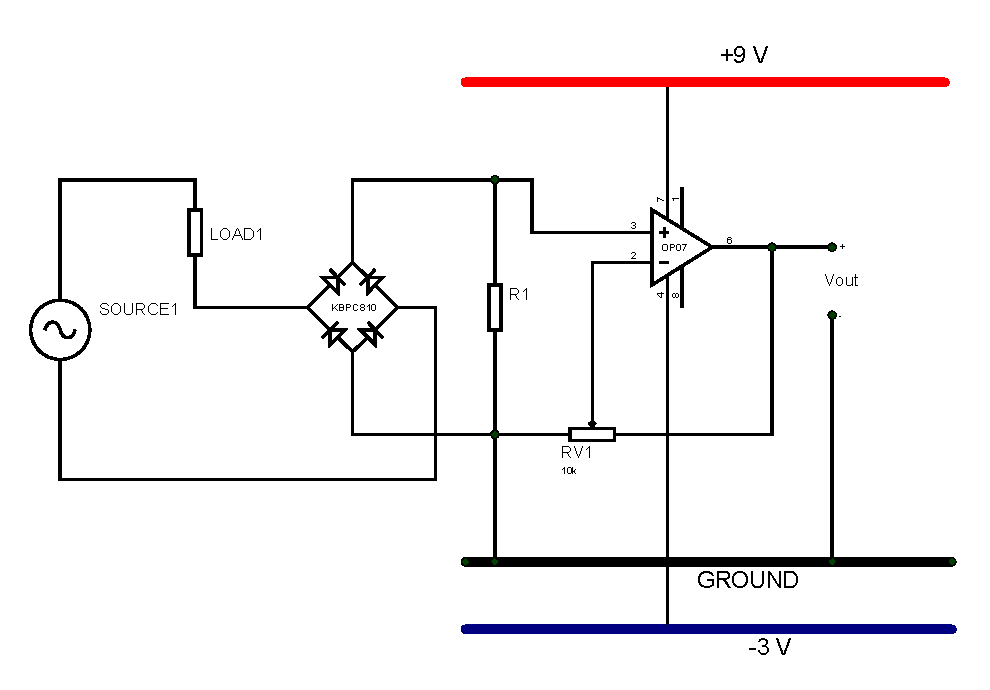
\includegraphics[width=.8\textwidth]{DIYCS.pdf}\\
    \caption{الدايرة}\label{fig:cir}
\end{figure}

\textbf{بص يا سيدى}:
\begin{enumerate}
    \item[أولاً] 
    الــ\textenglish{LOAD} اللى انت شايفه هو والــ\textenglish{SOURCE}:
    دول بيمثله أى حاجة شغال (تكيف، عسالة، ماتور، اى  حاجة\ldots )
    و المتوصلة بالفيشة (اللى هى الــ\textenglish{SOURCE} طبعا).

    \item[ثانياً] 
    الحتة ديه \textit{ظريفة} شوية، 
    دة \textenglish{Rectifier} شغلته أنه بيوحد إتجاه التيار اللى داخل على
    المقاومة الــ(\textenglish{0.1Ω})، و \textbf{خلى بالك} دة بيوحد التيار اللى داخل للمقاومة بس يعنى التيار و الجهد متغيرين عادى على الأحمال.

    \item[ثالثاً]
    {\large هيييييـــــــح}، \quad التيار أياً كان إتجاهه على الــ\textenglish{LOAD} 
    هايبفضل فى نفس الإتجاه على الــ\textenglish{0.1Ω}،
    و دة عشان الــ\textenglish{OP AMP} يقرأ الڤولت اللى على المقاومة دايماَ فى نفس الإتجاه، 
    الڤولت اللى على المقاومة بيبقا صغير و لذلك الــ\textenglish{OP AMP} 
    بيكبره بشكل مناسب، ممكن إحنا نستغل دة بقا براحتنا بالتغير فى الريوستات \textenglish{RV1} بحيث إننا نظبط الڤولت بشكل يناسب الأردوينو أو الــ\textenglish{ESB}.

    \item[رابعاً] 
    مابين كل الأنواع بتاعة الــ\textenglish{Operational Amplifier}
    إحنا لازم نختار نوع يتعامل مع الڤولت الصغير بطريقة مناسبة. هتلاقى معظم الــ\textenglish{Operational Amplifiers} 
    فيهم الــ\textenglish{Offset Volatge}\RTLfootnote%
    {الــ\textenglish{Offset Voltage} هو عبارة عن إزاحة صغيرة عن قيمة الجهد الداخل اللى بيكون عندها خرج الــ \textenglish{OP AMP} \textenglish{0V}. 
    شرحها على \hyperref{https://toshiba.semicon-storage.com/ap-en/semiconductor/knowledge/faq/linear_opamp/what-is-the-input-offset-voltage-of-an-op-amp.html}{}{}{ الموقع دة.}}
    حوالى \textenglish{5–10mV} و دة كتير طبعا.
    النوع \textenglish{OP07} بقا دة الــ\textenglish{Offset} بتاعه بيتقاس الــ\textenglish{$\mathrm{\mu V}$}
    عشان كدة هو مناسب لينا.

    \item[خامساً و أخيراً] 
    وديه بقا إسمها {\Large \textbf{غباوة}}. بس دة اللى أنا عملته، النقط اللى متوصلة بالارضى كلها \textenglish{node} 
    واحدة هتبقى متوصلة بالأردوينو هنا بقى هتلاقى بعض متشددين الــ\textenglish{safety} 
    هايقولوا لو حصل \textenglish{fault} ممكن يحصل مشاكل
    بس مصر كلها عايشة أهى قدامك و بقينا ١٠٠ مليون أو أكتر زى ما أنت شايف.{\fontspec{Arial}☺}
    كان المفروض يبقا فيه \textenglish{Isolation Transformer} مثلاً
    أو أى حاجة ممكن تعمل \textenglish{Isolation} بين 
    الدايرتين(الــ\textenglish{AC~220V} و الــ\textenglish{DC~12V})
    على سبيل المثال لو المقاومة \textenglish{R1 0.1Ω} خرجت من الدايرة ﻷاى سبب أو أتحرقت 
    الجهد اللى عليها هيبقى كبير جدا و أكيد هيبوظ الــ\textenglish{Amplifier} 
    عشان كدة الدايرة ديه عايزة حرص كويس، وطالما إحنا إتعاملنا مع الدايرة كلها بحرص مش هيحص حاجة بإذن الله.
\end{enumerate}

\subsection{حسبة الــ\textenglish{Gain}}

اللڤولت اللى على المقاومة \textenglish{1Ω R1} صغير بيبقا بتاع \textenglish{1V}. اللڤولت دة مش مناسب أنه يتقرى على الــ\textenglish{ESB} أو الأردوينو.
الــ\textenglish{Amplifier} المفروض أنه يكبر الڤولت اللى على المقاومة \textenglish{1Ω R1}

عشان نعرف نحسب الــ\textenglish{Gain} الصح بتاع الــ\textenglish{Amplifier} من الدايرة
ممكن نتخيل إن الريوستات \textenglish{RV1} عبارة عن مقاومتين \textenglish{R1, R2}.
\begin{figure}[!ht]
    \centering
    \begin{subfigure}{0.45\linewidth}
        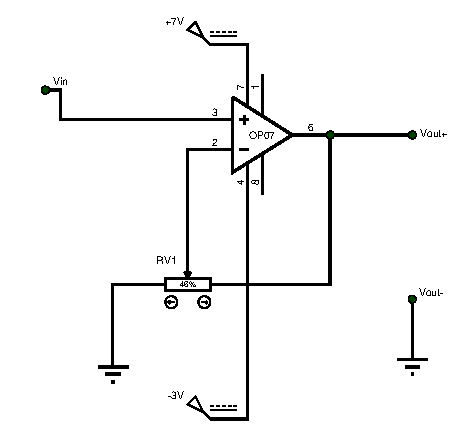
\includegraphics[width=\linewidth]{op amp cut.pdf}
        \caption{}
    \end{subfigure}
    \begin{subfigure}{0.45\linewidth}
        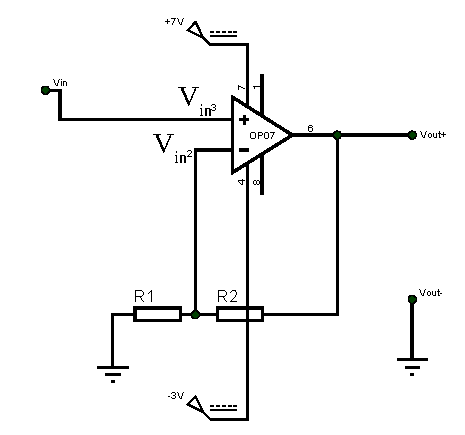
\includegraphics[width=\linewidth]{op amp cut exp.pdf}
        \caption{}
    \end{subfigure}
    \caption{}\label{fig:opampcut}
\end{figure}

فى حالة إن الــ\textenglish{Amplifier} مثالى هيبقى $\mathrm{V_{in^3} = V_{in^2}}$ وعندنا
\[\mathrm{ V_{in^2} = V_{out} \times \frac{R1}{R1+R2} }\]
يبقى 
\[\mathrm{ V_{in^3} = V_{out} \times \frac{R1}{R1+R2} }\]
يعنى
\begin{equation}
    \mathrm{  V_{out} = V_{in^3} \times \frac{R1+R2}{R1} = V_{in} \times \frac{R1+R2}{R1} }    
\end{equation}\label{eq:vout-in-rel}


\noindent يبقى إحنا ممكن نحدد قيمة الــ\textenglish{gain} بتاعنا عن طريق النسبة بين $\textstyle\mathrm{\frac{R1}{R1+R2}}$

الــ\textenglish{OP07} بيكبر من غير دايرة قيمة ضخمة جدا حوالى ٢٠٠ ألف مرة ضعف الجهد الداخل عشان كدة ممكن نعتبره قريب من أنه يكون مثالى،
وعموما معظم أنواع الــ\textenglish{Amplifier} ليها معامل تكبير ضخم

هو أنا جيبت الكلام دة من مكانين:
 \hyperref{https://www.electronics-tutorials.ws/opamp/opamp_3.html}{}{}{الموقع~دة}
 و الكتاب دة \\
 \hyperref{Behzad Razavi - Fundamentals of Microelectronics (2013, Wiley).pdf}{}{}{\textenglish{Behzad~Razavi,~Fundamentals~of~Microelectronics,~Second~Edition.~page~357\~{}359}} هتلاقى نسخة فيها الجزء المطلوب مع الحاجة


\subsection{حساب نسبة التكبير من تيار الأحمال}
إذا كانت مقاومة الأحمال هى $\mathrm{R_{LOAD}}$ و الجهد الفعال (${\mathrm{V_{RMS}} = 220 \mathrm{\ Volts}}$) أى أن 
($ \mathrm{V_{peak}} = \mathrm{V}_a \approx 311 \mathrm{\ Volts} $). يجب ظبط نسة التكبير لتحمل أقصى تيار لحظى أى ($\mathrm{V}_a$) بحيث عند هذا التيار 
يتولد أعلى جهد ممكن على دخل الــ\textenglish{ESB}. أعلى جهد عند أعلى تيار يؤدى الى أعلى دقة ممكنة.
يكون الجهد المطبق على الأحمال أقل من ${\mathrm{V_RMS}}$ بــ2 او 3 ڤولت نتيجة لوجود الــ\textenglish{Rectifier}.
\[\mathrm{V_{LOAD}} = \mathrm{V}_a - \mathrm{\underbrace{V_{drop}}_{3\ Volts}}\]
تضاف المقاومة $R_{sensor}$ على التوالى مع الاحمال لقياس التيار. يمكن حساب التيار كالآتى
\[\mathrm{I_{LOAD}} = \frac{\mathrm{V}_a-\mathrm{V_{drop}}}{\mathrm{R_{LOAD}+R_{sensor}}}\]
الجهد المتولد على المقاومة $\mathrm{R_{sensor}}$ هو الدخل للــ\textenglish{Amplifier} ($\mathrm{V_{in}} = V_{sensor}$).
يجب أن يتم تكبيره ليصل الى أقصى جهد من خرج الــ\textenglish{Ampilifer} عند مرور أعلى تيار كالآتى:
\[\mathrm{V_{out}} = G_a \cdot \mathrm{V_{in}} = G_a \cdot \mathrm{I_{LOAD}R_{sensor}} \]
حيث $G_a$ هو معامل التكبير. وإذا كان أقصى جهد لخرج الــ\textenglish{Amplifier} هو $\mathrm{V_{out\,max}}$ فإن:
\[G_a = \frac{\mathrm{V_{out}}}{\mathrm{V_{in}}} = \frac{\mathrm{V_{out\,max}}}{\mathrm{V_{sensor}}} %
      = \frac{\mathrm{V_{out\,max}}}{\mathrm{I_{LOAD}R_{sensor}}} \]  
من المعادلة \ref{eq:vout-in-rel}
\[\frac{R1+R2}{R1} = G_a\]
\begin{equation}
    \mathrm{ \frac{R1}{R1+R2} = \frac{\mathrm{I_{LOAD}R_{sensor}}}{\mathrm{V_{out\,max}}}}
\end{equation}


\section{توزيعة الجهود و التغذية}

عشاان نعرف نشغل الأجهز كل جهاز محتاج جهود مختلفة.
\begin{enumerate}
    \item الــ\textenglish{Amplifier} محتاج جهد من \textenglish{-3V} لـ\textenglish{+9V} عشان يشتغل.
    \item الــ\textenglish{ESP32} محتاجة \textenglish{5V} أو \textenglish{3.3V}.
    \item طبعا الأرضى جهده \textenglish{0V}.
\end{enumerate}

هنستخدم طريقة بسيطة: أعلى جهد فى الدايرة هو الــ\textenglish{9V} و أقل جهد هو \textenglish{-3V}. الفرق ما بينهم هو \textenglish{12V}.
مش مهم حاجة فى الــ\textenglish{supply} اللى هنستخدمه غير أنه يطلع فرق فى الجهود زى اللى إحنا عاوزينها.
بمعنى إن لو الــ\textenglish{supply} مثلاً بيطلع \textenglish{12V} هيبقى أقل جهد فى الدايرة
(الــ\textenglish{-3V}) 
هو السالب بتاع الــ\textenglish{supply} و الموجب هو الــ\textenglish{9V}. كدة مظبوط الفرق بين أعلى جهد و أقل جهد فى الدايرة هو \textenglish{12V}.
الجزئية اللى بتلفّف الدماغ الــ\textenglish{Ground} فين؟
الــ\textenglish{Ground} أعلى من الــ\textenglish{-3V} بــ\textenglish{3V} شيئ منطقى! الفكرة كلها أن الــ\textenglish{Ground}
دة نقطة فى الدايرة جهدها مفروض أنه بصفر عشان تقارن بقيت الجهود التانية بالنسبة ليه مش لأنه جهده فعلاً بصفر. المهم دايما فى الدايرة عندك هو فرق الجهود.
مثلا فى الشكل \ref{fig:vref} كل فروق الجهود ديه واحدة و كلهم نفس توزيعة الجهود و مناسبين لتشغيل الدايرة.

\begin{figure}[h]
    \centering
    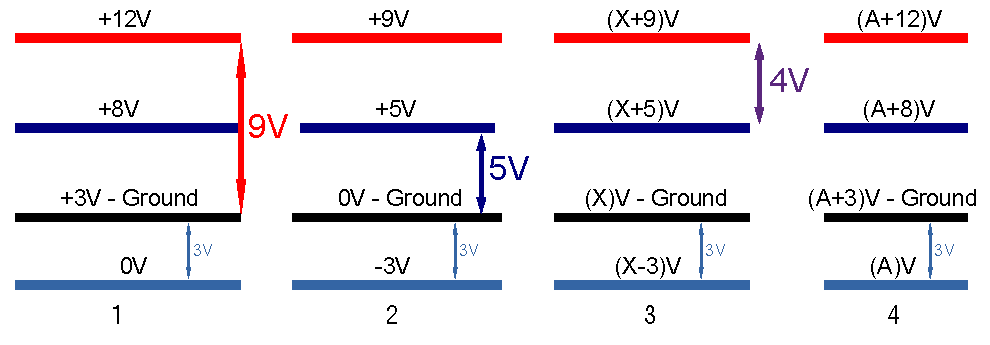
\includegraphics[width=0.7\textwidth]{vref.pdf}
    \caption{}\label{fig:vref}
\end{figure}

طيب إحنا عرفنا نطلع أكبر جهد و أصغر جهد لكن الجهو اللى فى النص بتطلع إزاى؟ بــ\textenglish{Regulator}. بشكل عام فى نوعين من الــ\textenglish{Regulator}:
\begin{itemize}
    \item \textenglish{Positive Regulator} \\
    معروف بياخد طرفين فرق الجهد مابينهم كبير بيطلع حهد ثابت بالنسبة للجهد الصغير. مثلاً
    \textenglish{8V} \textenglish{Positive Voltage Regulator} لو وصلته بــ\textenglish{12V} و \textenglish{0V}، هتلاقى الــ\textenglish{Regulator}
    بيطلع \textenglish{+8V} بالنسبة للــ\textenglish{0V} يعنى \textenglish{-4V} بالنسبة للــ\textenglish{12V} زى اول شكل فى الصورة \ref{fig:vref}
    \item \textenglish{Negative Regulator} \\
    بيطلع جهد ثابت بالنسبة للجهد الكبير. بمعنى إن الــ\textenglish{Regulator} بيطلع جهد أقل من أعلى جزء فى الدايرة بمقدار ثابت.
    مثلاً لو عندنا \textenglish{9V} \textenglish{Negative Voltage Regulator} لو وصلته بــ\textenglish{12V} و \textenglish{0V}، هتلاقى الــ\textenglish{Regulator}
    بيطلع \textenglish{-9V} بالنسبة للــ\textenglish{12V} يعنى \textenglish{+3V} بالنسبة للــ\textenglish{0V} زى اول شكل فى الصورة \ref{fig:vref}
\end{itemize}
\emph\strong{لاحظ}
إن معظم انواع الــ\textenglish{Regulator} بتوصل التيار فى إتجاه واحد بس الإتجاه التانى ممكن يحرقه.
الــ\textenglish{Positive Regulator} بيخرج تيار فقط و الــ\textenglish{Negative Regulator} بيدخله تيار فقط.
شرح أكتر فى \mbox{\hyperref{Linear Voltage Regulator.pdf}{}{}{المقال~ده~\textenglish{Linear~Voltage~Regulator.pdf}}~هتلاقيه~مع~الملفات}.

عشان نعمل الدايرة كناه محتايجن توزيعة الجهود زى اللى فى الشكل \ref{fig:vref}. و عشان نعملها هنستخدم 2 \textenglish{Voltage Regulator}. 
واحد \textenglish{Negative Regulator 9V} يستخدم كــ\textenglish{GROUND} و يبقى الفرق بينه و بين الــ\textenglish{12V} يبقى \textenglish{-9V}.
اما التانى فهو \textenglish{Positive Regulator 5V} هتركب من الــ\textenglish{Ground} اللى إحنا عملنها لغاية الــ\textenglish{12V}. 
و دة هيطلع جهد أعلى من الــ\textenglish{Ground} بــ\textenglish{5V}. دة بقا عشان يشغل الــ\textenglish{ESB}. و بكدة تكون إكتمل التوزيعة و هيبقا شكلها حاجة شبه الدايرة اللى \hyperref[fig:project scheme]{فالصورة ديه (صور \ref*{fig:project scheme})}

\begin{figure}[h]
    \centering
    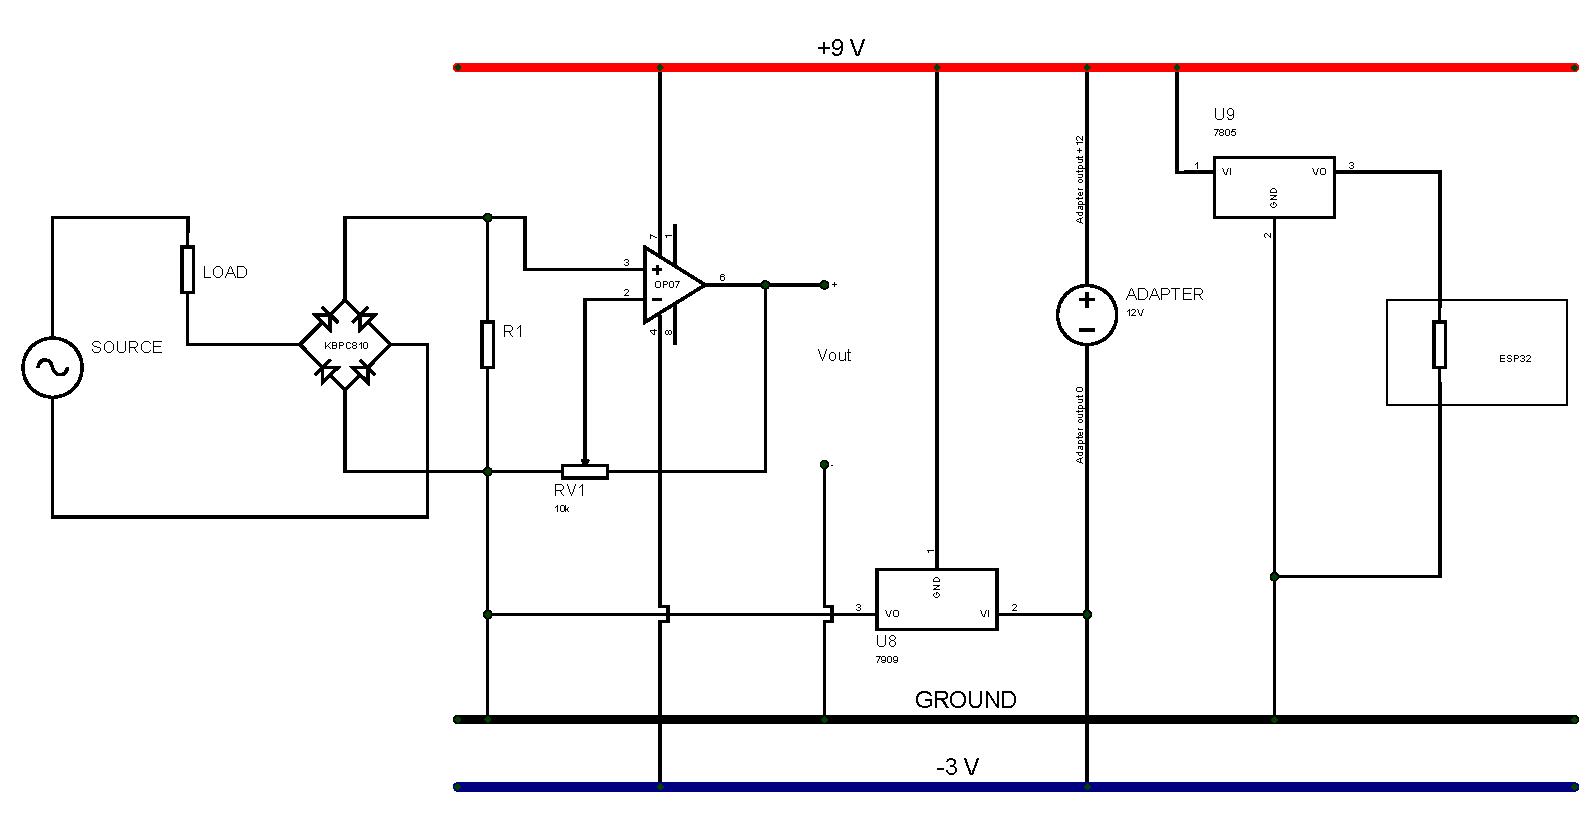
\includegraphics[width=\textwidth]{project scheme.pdf}
    \caption{}
    \label{fig:project scheme}
\end{figure}

فاضل حاجة واحد الــ\textenglish{Negative Voltage Regulator} بياخد الجهد العالى كــ\textenglish{Ground} و الجهد القليل كــ\textenglish{V\textsubscript{input}}.\\


\section{\textenglish{Relay Switching Cricuit}}

عشان نشغل الريلاى و نقفله أولاً محتاجين جهد \textenglish{12V} مش الــ\textenglish{3.3V} بتوع الــ\textenglish{ESP}.
ثانياً تيار الريلاى كبير ما ينفعش يطلع من الــ\textenglish{output pins ESB}.
يبقا إحنا عوزين نخلى الدايرة تشغل الريلاى بجهد \textenglish{12V}. أكيد عشان نعمل كدة محتاجين \textenglish{{\fontspec{Arial}♥}Transistor\fontspec{Arial}♥}.
الدايرة اللى أنا عرفت أعملها بتاخد 2 \textenglish{Transistor} و شكل الدايرة فى \hyperref[fig:rel swtch cir]{الصور ديه (الصورة \ref*{fig:rel swtch cir})}.
هتلاقى فى الصورة الــ\textenglish{Switch} بيعبر عن خرج الــ\textenglish{ESP}. و الــ\textenglish{BC558} دة \textenglish{Transistor \textit{PNP}}. 
الــ\textenglish{2N2222} دة \textenglish{Transistor \textit{NPN}}. أما الــ\textenglish{3.3V} فدول إحنا هانجيبهم من الــ\textenglish{ESB} نفسها.
لو بصيت على \hyperref[fig:ESP32PinDiagram]{الصورة \ref*{fig:ESP32PinDiagram}} اللى فيها توزيع الــ\textenglish{pin}ات هتلاقى من اول \textenglish{pin} ديه بتبقا \textenglish{3.3V pin}.
\\

\begin{figure}[h]
    \centering
    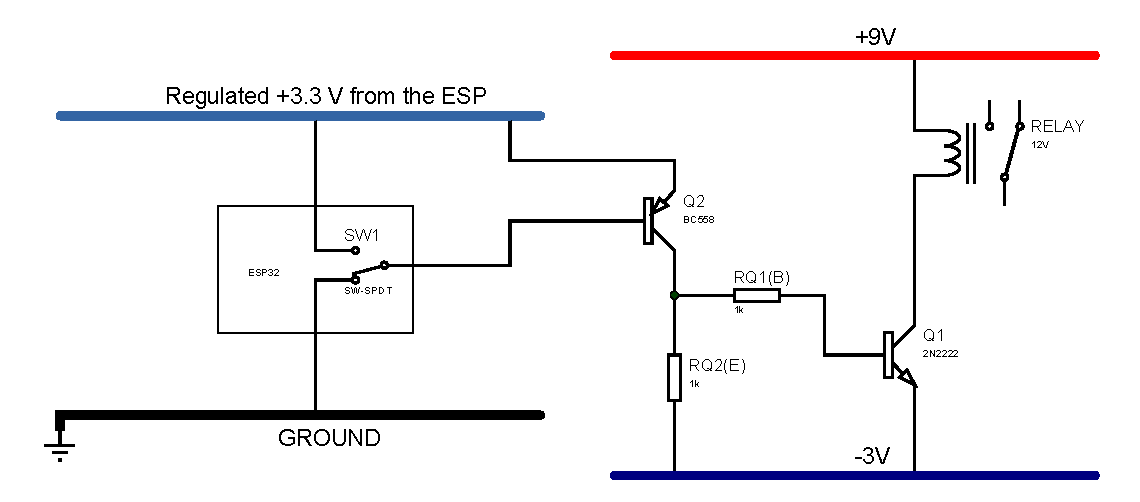
\includegraphics[width=\textwidth]{Switching Circuit.pdf}
    \caption{}\label{fig:rel swtch cir}
\end{figure}


عشان نفهم الرسمة محتاجين مراجعة سريعة على الفرق بين الــ\textenglish{\textit{PNP}} و الـ\textenglish{Transistor \textit{NPN}} كــسويتشات.\ \  
طيب \textenglish{Transistor \textit{NPN}} كان بيحتاج جهد الــ\textenglish{base} يبقى أعلى من الــ\textenglish{emitter} عشان يوصل، 
لو الــ\textenglish{base} اقل من الــ\textenglish{emitter} يبقى الــ\textenglish{cut off Transistor} و مش هيوصل،
وكان الــ\textenglish{collector} أعلى جهد فى الجهاز.
أما \textenglish{Transistor~\textit{PNP}} كان لازم الــ\textenglish{base} يبقى أقل من الــ\textenglish{emitter} عشان يوصل،
لو جهد \textenglish{base} أعلى من الــ\textenglish{emitter} يبقى الــ\textenglish{cut off Transistor} و مش هيوصل،
وكان الــ\textenglish{collector} أقل جهد فى الجهاز.

\strong{كفاية كلام نخش على الشغل فى ملف إسمه \textenglish{\texttt{"Switching Circuit.pdsprj"}} دة بقا هيفهمك الدايرة حلو بالــ\textenglish{simulation}.}


\section{\textenglish{The Mirco Controller (ESB)}}

هو فيه نوعين من الــ\textenglish{ESB}: \textenglish{ESB32} و \textenglish{ESP8266}. 
إحنا هانحتاج الــ\textenglish{ESB32} عشان هى اللى فيها \textenglish{pin}ات \textenglish{analog} تناسب
القرايات اللى بتطلع من الــ\textenglish{Ampilifer}.
هو في موقع شارحهم كويس 
\hyperref{https://www.circuitspecialists.com/blog/esp-microcontroller-quick-start-guide/}
{}{}{الموقع دة}.



لو بصيت على \hyperref[fig:ESP32PinDiagram]{صورة الــ\textenglish{pin diagram}} بتاعة الــ\textenglish{ESB32} هتلاقى إن فيها 
\textenglish{pin}ات 
كتير لونها \textenglish{\textcolor{green}{\textarabic{أخضر}}} 
ديه الــ\textenglish{pin}ات 
اللى ممكن تشتغل \textenglish{analog}. هى سعرها أغلى أنا عارف بس هى الأنسب لينا

\begin{figure}[h]
    \centering
    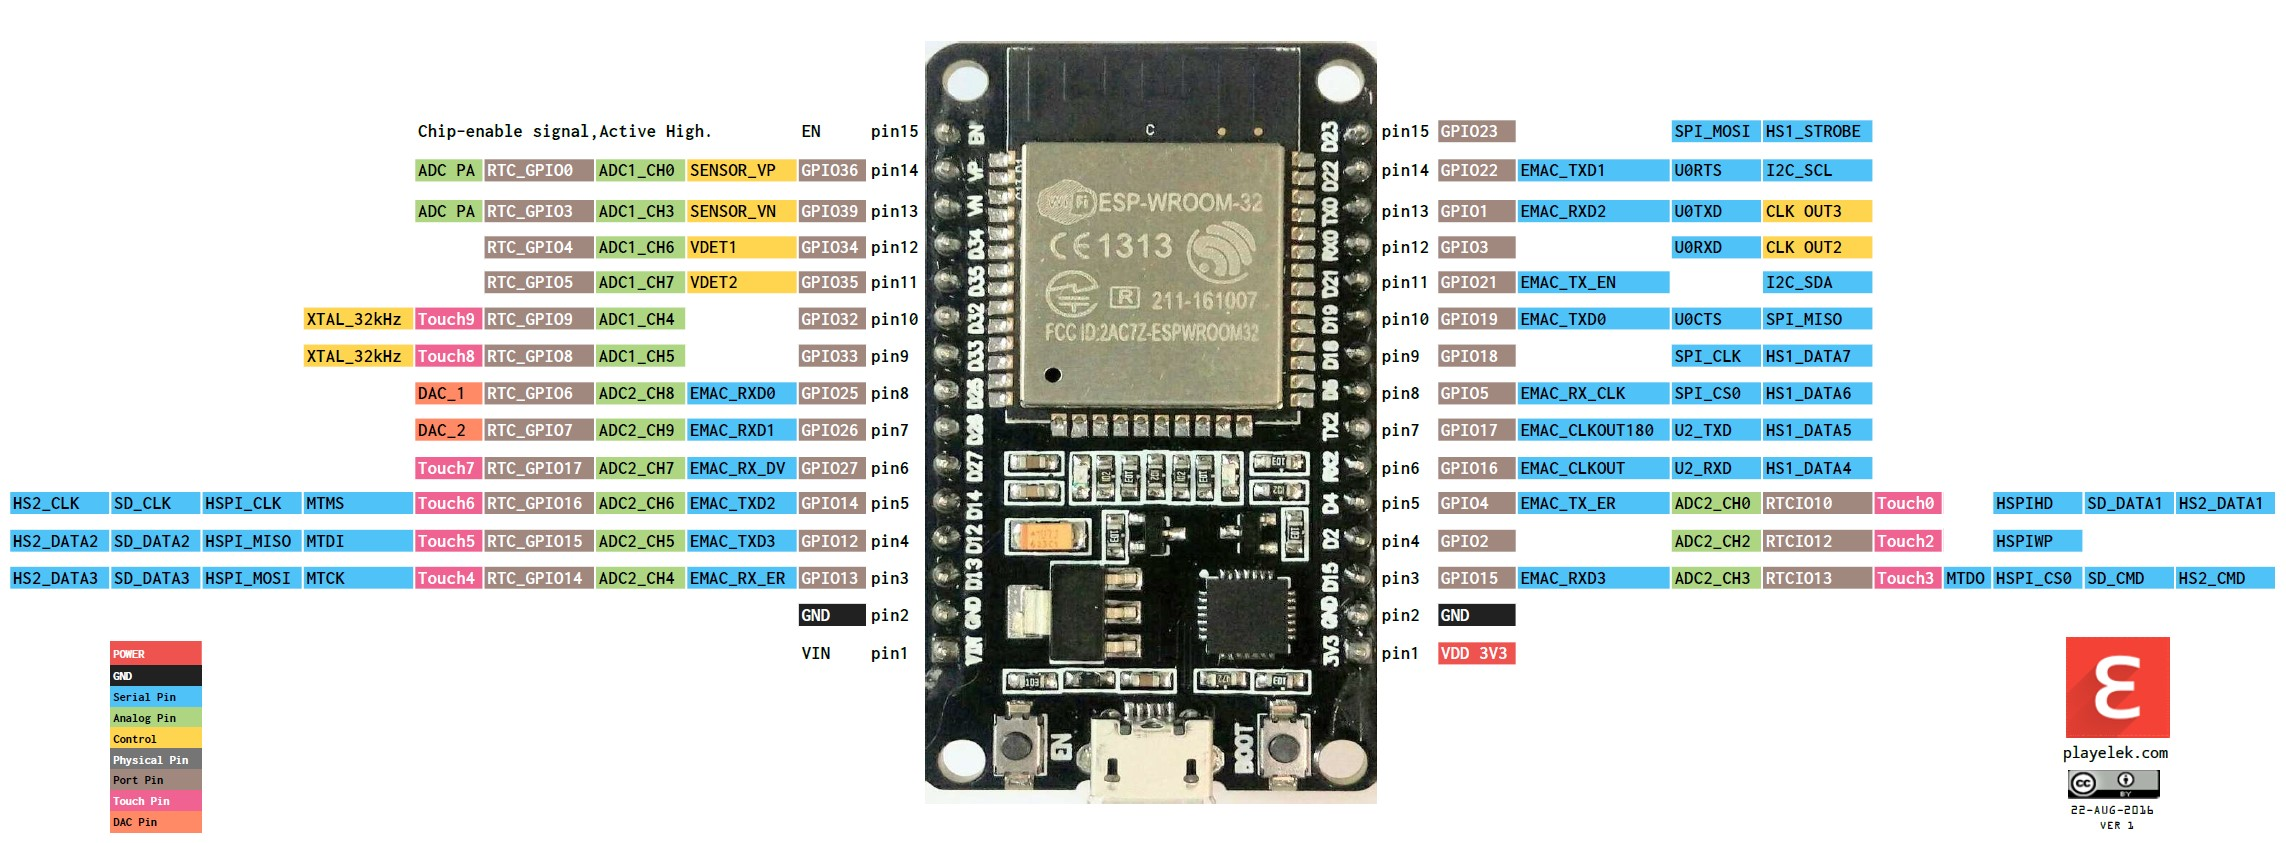
\includegraphics[width=0.9\textwidth]{ESB32 Pin diagram.jpg}
    \caption{\textenglish{ESB32 Pin Diagram}}\label{fig:ESP32PinDiagram}
    هتلاقى الصورة ديه مع باقى الملفات
\end{figure}

*ملحوظة هو فيه حل من غير الــ\textenglish{ESB32} بس دة عاوز أنك تركب دايرة أو جهاز بعد الــ\textenglish{Ampilifer}
عشان ينفع يتقرى بس طبعا دة أصعب من حيث الكود و من حيث الإنك تلاقى الجهاز أو الدايرة اللى ممكن تصمم بالشكل اللى أنت عاوزه



\section{إضافة \textenglish{Capacitor} لتنعيم القريات}
\needspace{144pt} \begin{wrapfigure}{l}{0.3\textwidth}
    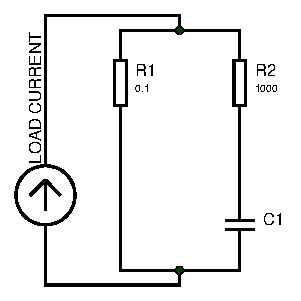
\includegraphics[width=0.3\textwidth]{smothing cap current and voltage approx .pdf}
    \caption{}\label{smcap}
\end{wrapfigure}
بص يا كوكو عشان أنا زهقت و ما حدش كدة كدة بيقرأ البتاع دة.
أولا إحنا حطينا الــ\textenglish{Capacitor} قبل الــ\textenglish{Amplifier} عشان الـنحية التانية التيار محدود و فى نفس الوقت الــ\textenglish{ESB} بيسحب تيار كبير شوية فهيطلع قرايات غلط، جربتها على
\textenglish{Proteus}. طيب ديه رسمة تقريب الجهد على الشمال. \par
تلاحظ إن النسبة بين المقاومتين \textenglish{1:10000} يعنى نسبة التيار اللى هيمشى فى المقاومة الكبيرة صغير جدا و بالتالى إحنا ممكن نقرب حسبة الجهد بإنه تيار الحمل فى المقاومة الصغيرة.\par
عشان نبقا واخدين بالنا؛ تيار الــ\textenglish{Source} كبيرا أصلا فالتيار اللى هتسحبه مقاومة \textenglish{1000Ω} دة مش هيعمل مشاكل فى حدود التيار و فعلياً بمجرد ما المكثف يشحن التيار اللى بيمر بيبقا شبه معدوم.

نخش بقا على الحسابات، هنا إحنا عاوزين التيار الجهد المتغير على المقاومة \textenglish{R1 0.1Ω} يبقى جهد ثابت عشان كدة هنستخدم الــ\textenglish{Capacitor} كــ\textenglish{Low Pass Filter (LPF)} 
هي ديه أصلا \textenglish{RC LPF} منها نطلع إن الــ\textenglish{Transfer Function}:
\[H(j\omega) = \frac{1}{1+ j\omega RC}\]
يعنى نسبة التكبير اللى هتحصل فى الدايرة \strong{للجزء المتغير }هى:
\[\abs{H(j\omega)} = \frac{1}{\sqrt{1+(\omega RC)^2}} = \frac{1}{\sqrt{(1+(2πfRC)^2}}\]
لو إحنا عاوزين نمنع تردد \textenglish{50Hz} يبقا إحنا عاوزين مثلا يكون $(\,\abs{H(j\omega)} = 2\%)$ شوية حسابات يطلع
\[ RC \ge 0.159 \ \ \text{\textenglish{ΩF}} = 159 \ \ \text{\textenglish{KΩμF}} \]

خلى بالك معنى إننا نخلى الــ\textenglish{Gain} بــ\textenglish{2\%} دة معناه إن فيه نسبة خطأ \textenglish{2\%} و دة بالنسبة للــ\textenglish{Sin Wave}
بس ديه أصلا \textenglish{Rectified Sin Wave} بس عموما لما جربت على بروتس بتطلع النتايج قريبة جداً و فى نفس الوقت الخطأ أقل بشوية كسور. \emph{منطقى!} 
بس هنا فيه شىء مهم ألا و هو إن الــ\textenglish{input} عبارة عن إنصاص \textenglish{Sin Wave} بتكرر \textenglish{100}مرة فى الثانية مش \textenglish{50}!
ودة معنا إننا محتاجين الــ\textenglish{Transfer Function} تبقا لــ\textenglish{100Hz} دة غير إن كدة كدة نسبة الخطأ بتبقا أصغر أصلا من المحسوبة فها\,نخليها 
\textenglish{3\%} بدل \textenglish{2\%} نطلع بقا بشكل المعادلة:
\[\abs{H(j\omega)} = \frac{1}{\sqrt{(1+(2π \times \underbrace{100}_{\mathclap{frequency}} \times RC)^2}}\]
يعنى :
\[ RC \ge 0.053 \ \ \text{\textenglish{ΩF}} = 53 \ \ \text{\textenglish{KΩμF}} \]
تلاحظ كدة إننا ممكن نستخدم \textenglish{RC} قيمتها أقل و دة يققل من قيمة الكثف اللى إنا محتاجين نجيبه.\par 

بالنسبة للــ\textenglish{Time Response} هنا بقا الموضوع يختلف هنا المطلوب هو إننا نعرف فى حالة تغير فى التيار المكثف هياخد وقت قد إيه 
(يشحن أو يفرغ) 
عشان التغير دة يتقرى.
طريقة بسيطة نقرب بيها العملية هى الــ\textenglish{Step Response} للــ\textenglish{RC Circuit} المعادلة ديه –جدعنة من عندى كدة أنا اللى جايبها– 
بتعبر عن العلاقة بين الــ\textenglish{Response} و \textenglish{Time} للدايرة
{\begin{equation*}
    R(t) = 1 - e^{(t/\tau)} = e^{(t/R\cdot C)} \tag*{\tiny \textenglish{(step response equation)}}\label{eq:step response 1st order}
\end{equation*}}
يبقا لو $RC = 0.053 \text{\textenglish{ΩF}}$ هيطلع إن عشان المكثف يوصل لــ\textenglish{98\%} من قيمة التيار الحقيقية هياخد \textenglish{207 mS}. الحقيقة إنا دة بيفرض إن الــ\textenglish{input}
عبارة عن \textenglish{Step Response} لكن الأصل إن الــ\textenglish{input} عبارة عن \textenglish{Rectified Sin Wave} الوقت بيبقى أطول بحوالى 
\textenglish{+25\%} من الوقت الأصلى لما جربتها على \textenglish{Proteus} \par
طيب لو دورت على \textenglish{RAM} هتلاقى إن المكثف المتاح \textenglish{100μF} و أنسب مقاومة تجاب هى \textenglish{1000Ω} نحسب بقا من جديد
الــ \textenglish{RC = 0.1} أكبر من المحسوبة بس لسة أصغر من الــ\textenglish{50Hz} و 
إيه هى القيمة الجديد لمعامل لتكبير الــ\textenglish{input} المتغير:
\[ \abs{H(h\omega)} = \frac{1}{\sqrt{(1+(2π\times 100 \times 0.1)^2}} = 0.0159134789711477 \] 
طبعا زى ما هو واضح من الأرقام مكثف سعة أكبر = تنعيم أكتر للإشارة.
طيب بس هنا الــ\textenglish{Time Response} هيبقى أبطأ من معادلة \hyperref[eq:step response 1st order]{الــ\textenglish{Step~Response}} 
يطلع إن الــ\textenglish{Step Response Time}
\[ T = 0.3912 \ \ (\mathrm{S}) \] 
طبعا محتاجين ناخد رقم أكبر من دة عشان الوقت الفعلى بيكون أكبر وليكن \textenglish{0.5S}\\
هنا بقا الدايرة هتبقى كالآتى
\begin{figure}[h]
    \centering
    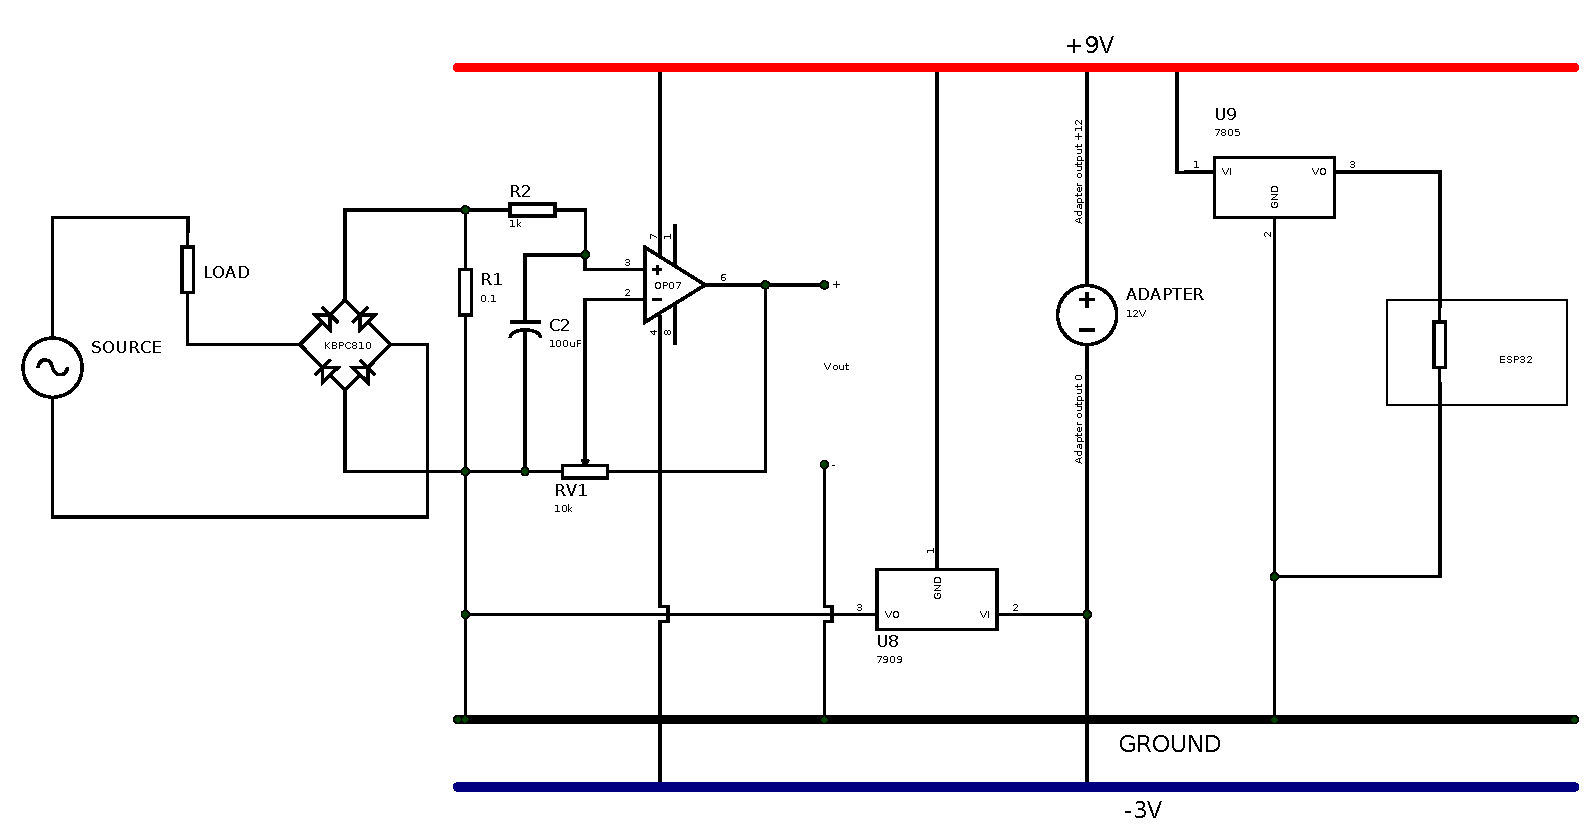
\includegraphics[width=\textwidth]{DIYCS with smothing cap.pdf}
    \caption{}\label{DIYCS with smothing cap}
\end{figure}

\section{التسعيرة}
هنا بقا أنا حاولت على قد ما أقدر أنا عملت دة كله عشان أحاول أخلى السعر معقول. كل حاجة و سعرها فى الجدول تحت.

\begin{english} \begin{tabular}{|r|c|r|}
    \hline 
      \textarabic{الوصف}
    & \textarabic{السعر}
    & \textarabic{البتاع}
    \\ \hline 
    4-diodes Bridge Rectifier 1.2 Voltage drop & 10 EGP & KBPC810R10
    \\
    10W Resistance, 10A & 2.5 EGP & Power Resistance 0.1Ω 
    \\
    1 Kohm ½W Vertical Square Cermet Potentiometer & 3.50 EGP & Potentiometer
    \\
    Ultralow Offset Voltage Operational Amplifiers & 7 EGP & OP07
    \\
    Positive Voltage Regulator 5V & 4 EGP & L7805CV
    \\
    Negative Voltage Regulator 9V & 4 EGP & L7909CV 
    \\
    Wall Adapter Fixed 12Vdc (1A) & 45 EGP & Adapter 12V
    \\
    5-pin relay with 10A AC/DC & 7 EGP & Relay 12V
    \\
    General Purpose \textit{PNP} Transistors & 0.50 EGP & BC558
    \\
    \textit{NPN} switching transistors & 0.50 EGP& 2N2222
    \\
    Fixed Carbon resistor ¼ watt, 15V, and 5\%\~{}10\% tolerance & 0.5 EGP & 1KΩ Carbon Resistor
    \\
    Polarized Electrolytic Capacitor 100μF 10v & 0.25 EGP & Polarized Capacitor 100μF
    \\
    & & \textarabic{٢ فيشة}
    \\
    & & \textarabic{سلوك}
    \\
    \hline
\end{tabular} \end{english}
\\ \vspace{12pt} 

\noindent *ملحوظة الــ\textenglish{KBPC810R10} دة \textenglish{Bridge Rectifier} مخصوص، 
المميز فيه أنه بيستحمل تيار عالى (حوالى \textenglish{35A}) و سعره معقول ١٠جم


\subsection{\textenglish{RAM e-shop}}
أنا دورت على الحاجة على \textenglish{RAM}.
\begin{itemize}
    \item 
    \hyperref{https://ram-e-shop.com/product/bridge-35aw-kbpc3510w/}{}{}{\textenglish{KBPC810R10}}
    \item 
    \hyperref{https://ram-e-shop.com/product/op07/}{}{}{\textenglish{Operational Amplifier OP07}}
    \item 
    \hyperref{https://ram-e-shop.com/product/10w-0-10ohm/}{}{}{\textenglish{Power Resistance 0.1Ω}}
    \item 
    \hyperref{https://ram-e-shop.com/product/pot-th-1k/}{}{}{\textenglish{Potentiometer 1KΩ}}
    \item
    \hyperref{https://ram-e-shop.com/product/7805-china/}{}{}{\textenglish{L7805CV}}
    \item  
    \hyperref{https://ram-e-shop.com/product/7909/}{}{}{\textenglish{L7909CV}}
    \item 
    \hyperref{https://ram-e-shop.com/product/adaptor-fixed-12v-1a/}{}{}{\textenglish{Adapter 12V}}
    \item 
    \hyperref{https://ram-e-shop.com/product/re1/}{}{}{\textenglish{Relay 12V}}
    \item 
    \hyperref{https://ram-e-shop.com/product/bc558/}{}{}{\textenglish{BC558}}
    \item 
    \hyperref{https://ram-e-shop.com/product/2n2222/}{}{}{\textenglish{2N2222}}
    \item 
    \hyperref{https://ram-e-shop.com/product/fixed-resistances-63/}{}{}{\textenglish{1KΩ Carbon Resistor}}
    \item 
    \hyperref{https://ram-e-shop.com/product/c-100u10v/}{}{}{\textenglish{Polarized Capacitor 100μF}}
    
    
    
\end{itemize}

\vspace*{\stretch{2}}

\begin{center}
    \Large \aracricfont 
\end{center} 

\vspace*{\stretch{1}}

\end{document}
